\documentclass{article}


% if you need to pass options to natbib, use, e.g.:
%     \PassOptionsToPackage{numbers, compress}{natbib}
% before loading neurips_2023
\PassOptionsToPackage{numbers, compress}{natbib}

% ready for submission
\usepackage{neurips_2023}


% to compile a preprint version, e.g., for submission to arXiv, add add the
% [preprint] option:
%     \usepackage[preprint]{neurips_2023}


% to compile a camera-ready version, add the [final] option, e.g.:
%     \usepackage[final]{neurips_2023}


% to avoid loading the natbib package, add option nonatbib:
%    \usepackage[nonatbib]{neurips_2023}


\usepackage[utf8]{inputenc} % allow utf-8 input
\usepackage[T1]{fontenc}    % use 8-bit T1 fonts
\usepackage{hyperref}       % hyperlinks
\usepackage{url}            % simple URL typesetting
\usepackage{booktabs}       % professional-quality tables
\usepackage{amsfonts}       % blackboard math symbols
\usepackage{nicefrac}       % compact symbols for 1/2, etc.
\usepackage{microtype}      % microtypography
\usepackage{xcolor}         % colors

\usepackage{algorithmic,algorithm}
\usepackage{amsmath}
\usepackage{amsopn}
\usepackage{amssymb}
\usepackage{amsthm}
\usepackage{bm}
\usepackage{color}
\usepackage{enumitem}
\usepackage{float}
\usepackage{graphicx}
\usepackage{mathrsfs}
\usepackage{mathtools}
\usepackage{multirow}
% \usepackage{natbib}
\usepackage{siunitx}
\usepackage{stfloats}
\usepackage{subfigure}
\usepackage{thmtools,thm-restate}
\usepackage{threeparttable}
\usepackage{verbatim}
\usepackage{wrapfig}
\usepackage{bbding}

\newtheorem{theorem}{Theorem}
\newtheorem{corollary}{Corollary}[theorem]
\newtheorem{proposition}{Proposition}
\newtheorem{lemma}[theorem]{Lemma}
\newtheorem{definition}[theorem]{Definition}
\newtheorem{condition}{Condition}
\newtheorem{hypothesis}{Hypothesis}

\newcommand{\xu}[1]{{\color{red} xu: #1}}
\newcommand{\yuan}[1]{{\color{blue} yuan: #1}}

\title{From Transformer to Sliceformer: \\Make Multi-Head Attention as Simple as Sorting}


% The \author macro works with any number of authors. There are two commands
% used to separate the names and addresses of multiple authors: \And and \AND.
%
% Using \And between authors leaves it to LaTeX to determine where to break the
% lines. Using \AND forces a line break at that point. So, if LaTeX puts 3 of 4
% authors names on the first line, and the last on the second line, try using
% \AND instead of \And before the third author name.


\author{Shen Yuan$^{1*}$\quad Hongteng Xu$^{1,2}$\thanks{The two authors have equal contributions. Hongteng Xu is the corresponding author.} \\
$^1$Gaoling School of Artificial Intelligence, Renmin University of China\\
$^2$Beijing Key Laboratory of Big Data Management and Analysis Methods\\
\texttt{shenyuan@ruc.edu.cn}\quad \texttt{hongtengxu@ruc.edu.cn}\\
  % examples of more authors
  % \And
  % Coauthor \\
  % Affiliation \\
  % Address \\
  % \texttt{email} \\
  % \AND
  % Coauthor \\
  % Affiliation \\
  % Address \\
  % \texttt{email} \\
  % \And
  % Coauthor \\
  % Affiliation \\
  % Address \\
  % \texttt{email} \\
  % \And
  % Coauthor \\
  % Affiliation \\
  % Address \\
  % \texttt{email} \\
}

\newcommand{\fix}{\marginpar{FIX}}
\newcommand{\new}{\marginpar{NEW}}

\begin{document}

\maketitle

\begin{abstract}
As one of the most popular neural network modules, Transformer plays a central role in many fundamental deep learning models, e.g., the ViT in computer vision and the BERT and GPT in natural language processing.
Although without strict theoretical supports, the effectiveness of the Transformer is often attributed to its multi-head attention (MHA) mechanism. 
In this study, we challenge this empirical opinion and discuss the limitations of the MHA mechanism, including the numerical issues caused by its softmax operation and the restricted capacity caused by the multi-head architecture. 
Considering the above issues and the recent development tendency of the attention layer, we propose an effective and efficient surrogate of the Transformer, called Sliceformer. 
Our Sliceformer replaces the MHA mechanism with an extremely simple ``slicing-sorting'' operation, i.e., projecting inputs linearly to a latent space and sorting them along different feature dimensions. 
We analyze the connections and differences between the proposed operation and the MHA mechanism and demonstrate the advantages of the corresponding Sliceformer on computational complexity, scalability, and numerical stability.
Experiments in the Long-Range Arena benchmark, image classification, and molecular analysis show that our Sliceformer achieves comparable or better accuracy with lower memory cost, faster speed, and better numerical stability than the Transformer and its variants. 
\end{abstract}

\section{Introduction}\label{sec:intro}
Transformer~\cite{vaswani2017attention} has been dominant in deep learning research for recent years. 
It works as a backbone module in many fundamental models, achieving outstanding performance in various application scenarios. 
Currently, the most successful language models like BERT~\cite{devlin2019bert} and GPT~\cite{brown2020language} are built based on the Transformer or its variants~\cite{child2019generating,dai2019transformer}, which outperforms classic recurrent neural network (RNN) architectures on both effectiveness and efficiency. 
In the field of computer vision, the Vision Transformers (ViTs)~\cite{dosovitskiy2021an,liu2021swin,arnab2021vivit} have achieved better performance in many image recognition and understanding tasks compared to convolutional neural networks (CNNs).
Recently, the Transformer-based models have been designed for the structured data in different applications, including the Informer~\cite{zhang2021informer} for time series broadcasting, the Graphormer~\cite{ying2021transformers} for molecular representation, the Set-Transformer~\cite{lee2019set} and Point-Transformer~\cite{zhao2021point} for point cloud modeling, and so on.
More and more cases show the tendency that the Transformer is becoming a natural and indispensable choice when developing deep learning models.

\begin{table}[t]
    \caption{A comparison for transformers and our sliceformer on their ``attention'' mechanisms. For simplification, we just show one attention head for each model, in which the input $\bm{X}\in\mathbb{R}^{N\times d}$, the value matrix $\bm{V}=\bm{X}\bm{W}_V\in\mathbb{R}^{N\times D}$, the query matrix $\bm{Q}=\bm{X}\bm{W}_Q\in\mathbb{R}^{N\times D}$, and the key matrix $\bm{K}=\bm{X}\bm{W}_K\in\mathbb{R}^{N\times D}$.}
    \label{tab:cmp}
    \centering
    \small{
    \begin{threeparttable}
    {\def\arraystretch{1.7}\tabcolsep=6pt
    \begin{tabular}{l|lll}
    \hline\hline
    Model & 
    $\text{Attention}(\bm{V};\bm{Q},\bm{K})$ & 
    Complexity & 
    Attention Structure \\
    \hline
    Transformer~\cite{vaswani2017attention}  & 
    $\text{Softmax}\left(\frac{\bm{Q}\bm{K}^{\top}}{\sqrt{D}}\right)\bm{V}$ & 
    $\mathcal{O}(DN^2)$ & 
    Dense + Row-stochastic\\
    SparseTrans~\cite{child2019generating} & 
    $\text{Local2D-Softmax}\left(\frac{\bm{Q}\bm{K}^{\top}}{\sqrt{D}}\right)\bm{V}$ & 
    $\mathcal{O}(DN^{1.5})$ &
    Sparse + Row-stochastic\\
    Longformer~\cite{beltagy2020longformer}   & 
    $\text{Local1D-Softmax}\left(\frac{\bm{Q}\bm{K}^{\top}}{\sqrt{D}}\right)\bm{V}$ &  
    $\mathcal{O}(DNL)$ &
    Sparse + Row-stochastic\\
    Reformer~\cite{kitaev2020reformer}     & 
    $\text{LSH-Softmax}\left(\frac{\bm{Q}\bm{K}^{\top}}{\sqrt{D}}\right)\bm{V}$ &  
    $\mathcal{O}(DN\log N)$ &
    Sparse + Row-stochastic\\
    CosFormer~\cite{zhen2022cosformer}    & 
    $(\bm{Q}_{\cos}\bm{K}_{\cos}^{\top}+\bm{Q}_{\sin}\bm{K}_{\sin}^{\top})\bm{V}$ & 
    $\mathcal{O}(\min\{DE_{QK},NE_{Q}\})$&
    Sparse\\
    Performer~\cite{choromanski2021rethinking}  & 
    $\phi_r(\bm{Q})\phi_r(\bm{K})^{\top}\bm{V}$ & 
    $\mathcal{O}(DNr)$ &
    Low-rank\\
    Linformer~\cite{wang2020linformer}    & 
    $\text{Softmax}\left(\frac{\bm{Q}\psi_r(\bm{K})^{\top}}{\sqrt{D}}\right)\psi_r(\bm{V})$ & 
    $\mathcal{O}(DNr)$ &
    Low-rank + Row-stochastic\\
    Sinkformer~\cite{sander2022sinkformers}   & 
    $\text{Sinkhorn}_{K}\left(\frac{\bm{Q}\bm{K}^{\top}}{\sqrt{D}}\right)\bm{V}$ & 
    $\mathcal{O}(KDN^2)$ &
    Dense + Doubly stochastic\\
    \hline
    \textbf{Sliceformer}  & 
    $\text{Sort}_{\text{col}}(\bm{V})$ & 
    $\mathcal{O}(DN\log N)$ &
    Sparse + Doubly stochastic\\
    \hline\hline
    \end{tabular}
    }
    \begin{tablenotes}
    \item[1] \footnotesize{``Local1D'' means considering the local data for a 1D sequence, while ``Local2D'' means considering the row-wise and column-wise local data for a sequence zigzagging in the 2D space. ``LSH'' denotes Locality-sensitive Hashing.}
    \item[2] \footnotesize{$\phi_r: \mathbb{R}^{D}\mapsto\mathbf{R}^r$, and $\phi_r(\bm{Q}),\phi_r(\bm{K})\in\mathbb{R}^{N\times r}$; $\psi_r: \mathbb{R}^{N}\mapsto\mathbf{R}^r$, and $\psi_r(\bm{K}),\psi_r(\bm{V})\in\mathbb{R}^{r\times D}$.}
    \item[3] $\bm{K}_{\cos}=\text{diag}(\{\cos\frac{\pi i}{2M}\}_{i=1}^{N})\text{ReLU}(\bm{K})$, $\bm{K}_{\sin}=\text{diag}(\{\sin\frac{\pi i}{2M}\}_{i=1}^{N})\text{ReLU}(\bm{K})$. So are $\bm{Q}_{\cos}$ and $\bm{Q}_{\sin}$. 
    $E_{QK}$ represents the number of nonzero elements in $\bm{Q}_{\cos}\bm{K}_{\cos}^{\top}$, while $E_Q$ represents the number of nonzero elements in $\bm{Q}_{\cos}$.
    \item[4] ``$\text{Sinkhorn}_{K}$'' means applying $K$-step Sinkhorn iterations.
    \item[5] Note that, our Sliceformer does not need the ``multi-head'' architecture because of the simplicity of sorting.
    \end{tablenotes}
    \end{threeparttable}
}
\end{table}

The popularity of the Transformer reflects the ``hegemony'' of the multi-head attention (MHA) mechanism~\cite{vaswani2017attention} behind it, which might be questionable in our opinion.
In particular, without strict theoretical support, the effectiveness of the Transformer is often attributed to the MHA mechanism.
This empirical but dominant opinion impacts the design and modification of the Transformer significantly.
As shown in Table~\ref{tab:cmp}, many efforts are made to $i)$ improve the efficiency of MHA, e.g., designing sparse or low-rank attention maps~\cite{child2019generating,kitaev2020reformer,wang2020linformer}, and $ii)$ enhance the interpretability of MHA, e.g., providing new understandings through the lens of kernel theory~\cite{tsai2019transformer,zhen2022cosformer} and optimal transport~\cite{tay2020sparse,sander2022sinkformers}.
Although some variants of Transformer challenge the sufficiency of MHA~\cite{dong2021attention,gu2021efficiently,ma2022mega}, they still take the MHA as a necessary module in their architectures. 
On the contrary, little attention is paid to studying the rationality and necessity of the MHA itself or, more ambitiously, replacing the MHA with a new surrogate. 
Recently, some work replaces the MHA with some other architectures, e.g., RNN~\cite{katharopoulos2020transformers} and MLP~\cite{tolstikhin2021mlp}, for specific tasks. 
However, they still reuse existing neural network layers rather than design a new and general module with a simpler architecture, better effectiveness, and higher efficiency.


In this study, we challenge the MHA mechanism in discriminative learning tasks, replacing it with an extremely simple ``slicing-sorting'' operation and, accordingly, developing a surrogate of the Transformer, called Sliceformer. 
Our work is motivated by two points: the drawbacks of the current MHA and the possibly-desired functionality reflected by its development tendency. 
Firstly, we attribute the MHA's poor scalability and numerical instability to the usage of the softmax operation and point out the potential loss of flexibility caused by the multi-head structure. 
Secondly, revisiting the development of the MHA and its variants, we summarize the tendency is pursuing multiple differentiable, sparse, and doubly-stochastic attention maps for projected samples. 
Based on the analysis above, we propose the ``slicing-sorting'' operation, which projects samples linearly to a latent space and sorts them along different feature dimensions. 
Replacing the MHA mechanism in a Transformer with the slicing-sorting operation leads to the proposed Sliceformer.

\begin{wrapfigure}{r}{0.5\textwidth}
  \centering
    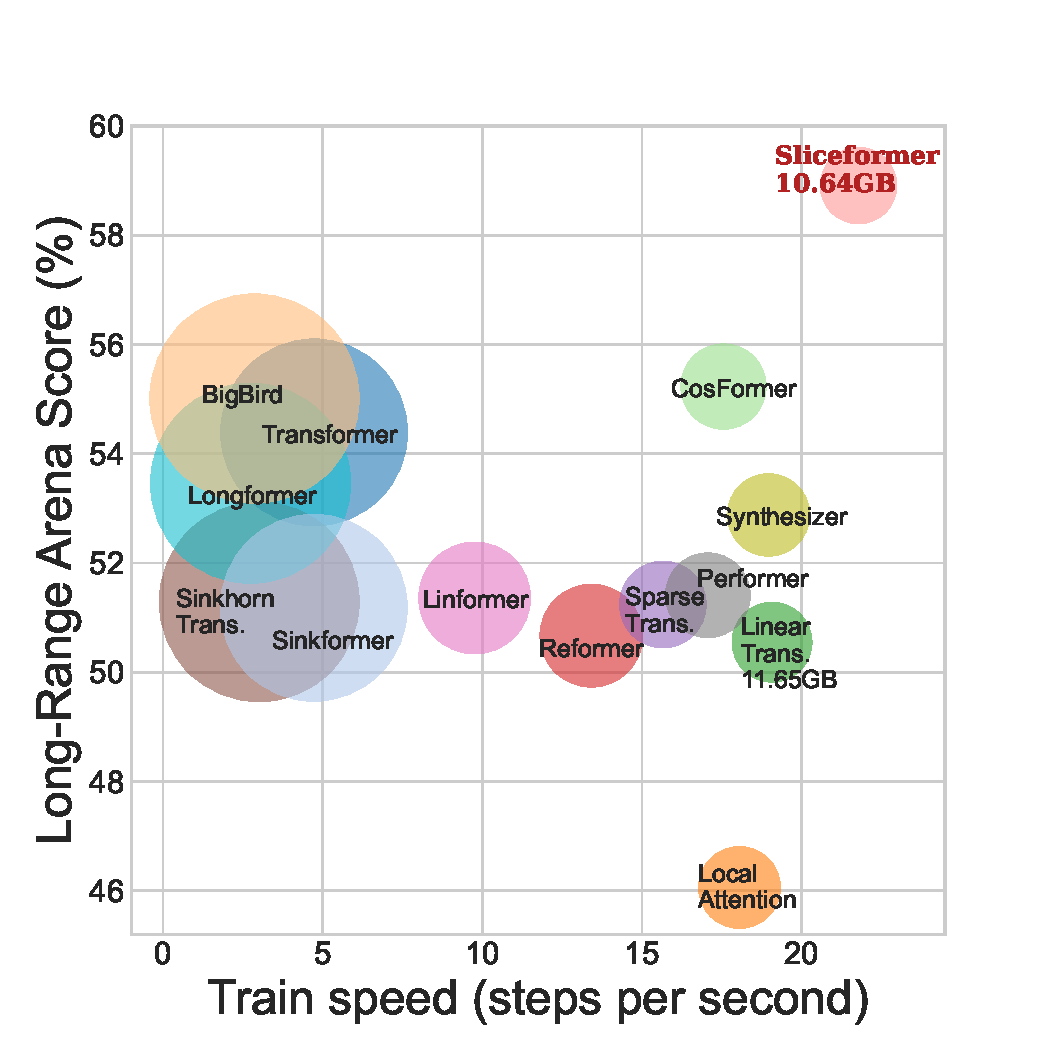
\includegraphics[width=0.46\textwidth]{figures/lra-3.pdf}
    \caption{The comparison for various Transformers and our Sliceformer on the LRA benchmark. 
    The length of sequence is 3K.
    The x-axis corresponds to the number of training steps per second. 
    The y-axis corresponds to the average score (\%) on the LRA benchmark.
    The peak memory usage of each model is represented as the area of the corresponding circle. 
    For a better comparison, the values (GB) of the top-2 models are shown.}
    \label{fig:cmp}
\end{wrapfigure}

% \begin{figure}[t]
%     \centering
%     \includegraphics{example-image-a}
%     \caption{The comparison for various Transformers and our Sliceformer. 
%     The x-axis corresponds to the number of steps per second, indicating the speed of the models. 
%     The y-axis corresponds to the average score on the LRA benchmark for each model.
%     The size of each model is represented by the size of the corresponding circle.}
%     \label{fig:cmp}
% \end{figure}

As shown in Table~\ref{tab:cmp}, our slicing-sorting operation only preserves the linear map from the input $\bm{X}$ to the value matrix $\bm{V}$. 
In addition, because of the simplicity of sorting, we do not need to design the ``multi-head'' concatenation architecture --- concatenating different linear maps is equivalent to increasing the columns of $\bm{W}_V$ directly. 
Therefore, the corresponding Sliceformer has fewer parameters and lower computational complexity compared to the Transformer and its variants. 
We analyze the connections and differences between the proposed slicing-sorting operation and the MHA mechanism and discuss its rationality in-depth. 
Specifically, we find that although abandoning the MHA mechanism, the slicing-sorting operation actually replaces the attention maps with a set of permutation matrices that are friendly to the backpropagation and have the sparsity and doubly-stochastic property. 
We test our Sliceformer in the well-known Long-Range Arena (LRA) benchmark. 
As shown in Figure~\ref{fig:cmp}, compared to the Transformer and its variants, our Sliceformer achieves superior performance with less memory cost and runtime. 
Moreover, through more analytic experiments, we demonstrate the numerical stability of our Sliceformer and its potential to large-scale classification problems.  
More details can be found in the following experimental section.


\section{Related Work}\label{sec:related}
Transformer~\cite{vaswani2017attention} is a powerful sequential model friendly to parallel computing. 
Since it was proposed, Transformer has become the critical module of many large language models, e.g., BERT~\cite{devlin2019bert}, Transformer-XL~\cite{dai2019transformer}, and GPT~\cite{brown2020language}. 
Besides texts, Transformer is also applied to other sequences, e.g., the Music Transformer~\cite{huang2018music} for music modeling, the Informer~\cite{zhang2021informer} for time series broadcasting and the Transformer Hawkes process~\cite{zuo2020transformer} for event sequence prediction. 
For non-sequential data like images, the Vision Transformer (ViT)~\cite{dosovitskiy2021an} and its variants~\cite{liu2021swin,chen2021visformer} take the patches of images as a sequence and extract image representations accordingly, which outperform convolutional neural networks (CNNs) in image classification.
Nowadays, Transformer is being introduced for structured data modeling, e.g., the Graphormer~\cite{ying2021transformers} for molecules, the Set-Transformer~\cite{lee2019set} for point clouds, and the Mesh Transformer~\cite{lin2021mesh} for 3D meshes. 
The more applications the Transformer has, the more significant it is to study its architecture, especially its MHA mechanism. 

It has been known that the classic MHA mechanism suffers from high computational complexity, poor scalability, and numerical instability for long sequences. 
As shown in Table~\ref{tab:cmp}, many efforts have been made to overcome these issues. 
The SparseTrans in~\cite{child2019generating} and the Longformer in~\cite{beltagy2020longformer} compute local attention maps based on the sub-sequences extracted by sliding windows, which leads to sparse global attention maps.
Some other models sparsify the key and query matrices directly by the locality-sensitive hashing (LSH)~\cite{kitaev2020reformer} or the ReLU operation~\cite{zhen2022cosformer}. 
Besides pursuing sparse attention maps, another technical route is constructing low-rank attention maps. 
The Performer~\cite{choromanski2021rethinking} reduces the feature dimension (the column number) of the query and key matrices, while the Linformer~\cite{wang2020linformer} reduces the sample dimension (the row number) of the key and value matrices. 

In addition to simplifying the computation of the attention maps, some work provides new understandings of the attention mechanism. 
The work in~\cite{tsai2019transformer} treats the attention map as a normalized linear kernel and revisits the vanilla Transformer through different kernels.
The Performer~\cite{choromanski2021rethinking} and the CosFormer~\cite{zhen2022cosformer} introduce additional mappings for the query and key matrices and consider their linear kernels in the latent spaces.
Recently, the work~\cite{sander2022sinkformers} reports an interesting phenomenon that the attention map tends to be doubly stochastic during training. 
Accordingly, it implements the attention map as an optimal transport through the Sinkhorn-Knopp algorithm~\cite{sinkhorn1967concerning}. 
Note that although providing these new understandings, these Transformer variants fail to design new model architectures that overcome the MHA's issues.

\section{Proposed Sliceformer}\label{sec:model}
\subsection{The Design Principle Guided by Two Hypotheses}
Typically, given an input $\bm{X}\in\mathbb{R}^{N\times d}$, where $N$ indicates the length of a sequence or the size of a sample set and $d$ is the input feature dimension, an attention layer first obtains the value, query, and key matrices by linear maps, i.e., $\bm{V}=\bm{X}\bm{W}_V\in\mathbb{R}^{N\times D}$, $\bm{Q}=\bm{X}\bm{W}_Q\in\mathbb{R}^{N\times D}$, and $\bm{K}=\bm{X}\bm{W}_K\in\mathbb{R}^{N\times D}$, and then projects $\bm{V}$ as follows:
\begin{eqnarray}\label{eq:att}
\begin{aligned}
    \text{Attention}(\bm{V};\bm{Q},\bm{K}):=\bm{P}(\bm{Q},\bm{K})\bm{V}.
\end{aligned}
\end{eqnarray}
Here, we take $\bm{V}$ as the input of the layer, and $\bm{P}(\bm{Q},\bm{K})\in\mathbb{R}^{N\times N}$ is the attention map parametrized by $\bm{Q}$ and $\bm{K}$, which can be implemented by various models (e.g., those shown in Table~\ref{tab:cmp}). 
The multi-head attention layer applies a group of linear maps, i.e., $\theta=\{\bm{W}_{V,m},\bm{W}_{Q,m},\bm{W}_{K,m}\in\mathbb{R}^{d\times D}\}_{m=1}^{M}$, to construct $M$ attention layers and concatenates their outputs, i.e.,
\begin{eqnarray}\label{eq:mha}
\begin{aligned}
    &\text{MHA}_{\theta}(\bm{X}) := \text{Concat}_{\text{row}}(\{\text{Attention}(\bm{V}_m;\bm{Q}_m,\bm{K}_m)\}_{m=1}^{M})\in\mathbb{R}^{N\times MD},\\
    &\text{where}~\bm{V}_m=\bm{X}\bm{W}_{V,m},~\bm{Q}_m=\bm{X}\bm{W}_{Q,m},~\text{and}~\bm{K}_m=\bm{X}\bm{W}_{K,m},~\forall m=1,...,M.
\end{aligned}
\end{eqnarray}
In this study, we analyze the architectures of the above multi-head attention layer used in different models and propose the following two hypotheses to guide our model design. 

Firstly, as Figure~\ref{fig:cmp}, the following experiments, and the results in~\cite{beltagy2020longformer,gu2021efficiently,zhen2022cosformer,ma2022mega} show, the models applying sparse attention maps, e.g., CosFormer and Longformer, can achieve competitive performance and higher efficiency than the vanilla Transformer. 
On the contrary, although imposing low-rank structures on the attention maps can also reduce the computational complexity, it seems to harm the performance --- the gaps between the vanilla Transformer and the models using low-rank attention maps are significant on the LRA benchmark. 
In our opinion, a potential reason for this phenomenon is that when $\text{rank}(\bm{P})\ll N$, the rank of the output embeddings $\text{MHA}_{\theta}(\bm{X})$ is likely to be smaller than $N$. 
Such linear dependency may limit the representation power of the output embeddings.
In addition, the work in~\cite{sander2022sinkformers} shows that in various discriminative learning tasks, the attention maps tend to be doubly stochastic (i.e., $\bm{P}\bm{1}_N=\bm{1}_N$ and $\bm{P}^{\top}\bm{1}_N=\bm{1}_N$) during training. 
Accordingly, the Sinkformer designs the attention maps based on the Sinkhorn-Knopp algorithm~\cite{sinkhorn1967concerning} and makes them doubly stochastic strictly, achieving better performance than the vanilla Transformer. 
Based on the above analysis, we propose a hypothesis on the desired structure of attention map as follows:
\begin{hypothesis}\label{hypo:1}
A desired attention map $\bm{P}$ should be full-rank, sparse, doubly stochastic, and applicable for the backpropagation.
\end{hypothesis}
Note that we do not restrict the desired attention map to be parametric. 
In other words, the query and key matrices might be unnecessary as long as the attention map has the desired structure and can be updated during training. 
Additionally, Hypothesis~\ref{hypo:1} challenges the rationality of the softmax operation commonly used in many Transformer models. 
Without any additional data preprocessing like LSH~\cite{kitaev2020reformer} or sliding windows~\cite{beltagy2020longformer,child2019generating}, the softmax operation always provides us with dense attention maps, which disobeys the hypothesis. 
What is worse, with the increase of data length $N$, the softmax operation often leads to over-smoothed normalization results and suffers from numerical instability issues.\footnote{Take the softmax function in PyTorch as an example. 
Through analytic experiments, we find that while the softmax operation should be permutation-equivariant, i.e., $\text{Softmax}_{\sigma}(\bm{x})=\text{Softmax}(\bm{x}_{\sigma})$ for an arbitrary vector $\bm{x}$ and an index permutation $\sigma$, such a fundamental property cannot be held in practice. 
The design of the experiment is given in Appendix~\ref{app:numerical}.}
In summary, Hypothesis~\ref{hypo:1} is not only about the desired structure of the attention map, but it also provides us with some guidance on our model design --- the parameterization of the attention map might be unnecessary, and the usage of softmax should be avoided. 

The second hypothesis is about the necessity of the multi-head architecture. 
On the one hand, the multi-head attention layer projects the input to different latent spaces and applies one attention map to each value matrix, as shown in~\eqref{eq:mha}. 
This multi-head architecture can increase the model capacity greatly~\cite{vaswani2017attention}, which embeds the input from different views. 
On the other hand, in~\eqref{eq:att}, the features within a value matrix, i.e., the columns of $\bm{V}$, share the same attention map $\bm{P}$, such that we only need to compute one attention map for $D$ features. 
The above observations reveal that the multi-head attention balances model capacity and computational complexity. 
In particular, given $MD$ features $\{\bm{V}_m\in\mathbb{R}^{N\times D}\}_{m=1}^{M}$, computing a specialized attention map for each feature can maximize the model capacity but leads to high computational complexity.
On the contrary, computing one attention map shared by all the features can minimize the complexity but limits the model capacity at the same time.
The solution of the multi-head attention layer is to group the features by $M$ heads and let the features in the same head share the same attention map. 
Based on the analysis above, we propose the following hypothesis: 
\begin{hypothesis}\label{hypo:2}
The multi-head architecture aims to achieve a trade-off between model capacity and computational complexity. 
It might be unnecessary if we can find a surrogate that simultaneously has high capacity and low complexity.
\end{hypothesis}
The second sentence in Hypothesis~\ref{hypo:2} indicates the motivation of our model design --- if we can compute a specialized attention map for each feature with low computational cost, such an operation might be comparable, even superior, to the current MHA mechanism.


\subsection{Slicing-sorting and Its Advantages}
The above two hypotheses motivate us to design the proposed slicing-sorting operation and accordingly, the Sliceformer. 
As shown in Table~\ref{tab:cmp}, our slice-sorting operation is extremely simple: projecting the input linearly to a latent space and sorting each feature, i.e.,
\begin{eqnarray}\label{eq:ss}
\begin{aligned}
    \text{SliceSort}(\bm{X}) := \text{Sort}_{\text{col}}(\underbrace{\bm{X}\bm{W}_V}_{\bm{V}}) = \text{Concat}_{\text{row}}(\{\bm{P}_i\bm{v}_i\}_{i=1}^{MD}) \in\mathbb{R}^{N\times MD},
\end{aligned}
\end{eqnarray}
where $\bm{W}_V\in\mathbb{R}^{d\times MD}$ is the projection matrix,\footnote{Here, we set the number of columns in $\bm{W}_V$ to be $MD$, such that the output has the same shape with the output of MHA.} and $\bm{V}=\bm{XW}_V$. 
Here, we call each column of $\bm{V}$ a ``slice'', denoted as $\bm{v}_i$ for $i=1,...,MD$. 
Each slice corresponds to the projection result of $N$ $d$-dimensional samples in a 1D space. 
As shown in~\eqref{eq:ss}, sorting a slice $\bm{v}_i$ corresponds to the multiplication between a permutation matrix $\bm{P}_i$ and the slice, and accordingly, our slicing-sorting operation concatenates all sorted slices as the output.  


\xu{Stop here.}

Why not use identity matrix: satisfy H1 but disobey H2.

Add a table to compare different maps under H1+H2.

\xu{Explain how to deal with position embedding.}

To overcome the drawbacks of softmax, existing Transformer models either reduce the size $N$~\cite{kitaev2020reformer,beltagy2020longformer,child2019generating} or apply other operations~\cite{tsai2019transformer,zhen2022cosformer}. 
However, reducing the size $N$ limits the representation power of the models for long sequence, and the other operations may not generate full-rank and doubly-stochastic attention maps.

\section{Experiments}\label{sec:exp}
We demonstrate the effectiveness and efficiency of our Sliceformer through comprehensive comparative and analytic experiments. 
In particular, we first compare our Sliceformer to Transformer and its representative variants on the Long Range Arena benchmark~\cite{tay2021long} and empirically verify the rationality of our slicing-sorting operation. 
Then, we implement ViT~\cite{dosovitskiy2021an} by our Sliceformer and test its performance and permutation-invariance in image classification tasks. 
Finally, we impose our slice-sorting operation on Graphormer~\cite{ying2021transformers}, leading to a Sliceformer for graph-structured data. 
This model achieves comparable performance in molecular representation with fewer parameters, demonstrating the universal applicability of our slice-sorting attention layer.
\textbf{Representative results are shown below. More results and implementation details are in the supplementary file. 
}


\subsection{Long Range Arena Benchmark}
Long Range Arena (LRA) is a benchmark designed to evaluate models for long sequence scenarios~\cite{tay2021long}, which consists of six discriminative learning tasks, including ListOps~\cite{nangia2018listops}, byte-level text classification~\cite{maas2011learning}, byte-level document retrieval~\cite{radev2013acl}, and three image classification tasks on CIFAR-10~\cite{krizhevsky2009learning}, Pathfinder~\cite{linsley2018learning},\footnote{Pathfinder is an image classification task: given a set of gray-level images, each of which plots two points and several curves, the model aims to recognize whether there exists a path connecting the points in each image.} and Pathfinder-X (a longer and more challenging version of Pathfinder). 
In the three image classification tasks, each image is formulated as a sequence of pixels.
We test our Sliceformer on the LRA benchmark and compare it to other Transformer-based models on both prediction accuracy and computational efficiency. 
In each task, our Sliceformer is trained to represent each input sequence through the embedding in the ``CLS'' position. 
For a fair comparison, we implement all the models based on JAX~\cite{bradbury2018jax} and strictly follow the benchmark's default data processing and experimental design.
In each task, our Sliceformer is the same as the other models on the number of layers and the dimension of hidden variables. 
Hence, its model parameters are fewer because of abandoning the ``query-key-value'' attention architecture. 
All the models are trained on 4 NVIDIA 3090 GPUs. 




\begin{table}[t]
  \centering
  \caption{The comparison for various models on the LRA benchmark. 
  ``FAIL'' means the training process fails to converge.
  In each column, we bold the best result and underline the second best one.}
  \small{
    \begin{tabular}{l|cccccc|c}
    \toprule
    \multicolumn{1}{c|}{Model} & ListOps & Text  & Retrieval & Image & Path  & Path-X & Avg. Acc (\%)\\
    \midrule
    Transformer~\cite{vaswani2017attention} & 36.37 & 64.27 & 57.46 & 42.44 & 71.40 & FAIL  & 54.39 \\
    \midrule
    Local Attention~\cite{tay2021long} & 15.82 & 52.98 & 53.39 & 41.46 & 66.63 & FAIL  & 46.06 \\
    Linear Trans.~\cite{katharopoulos2020transformers} & 16.13 & \textbf{65.90} & 53.09 & 42.34 & 75.30 & FAIL  & 50.55 \\
    Reformer~\cite{kitaev2020reformer}  & 37.27 & 56.10 & 53.40 & 38.07 & 68.50 & FAIL  & 50.67 \\
    Sinkformer~\cite{sander2022sinkformers} & 30.70 & 64.03 &  55.45 & 41.08 & 64.65 & FAIL & 51.18 \\
    Sparse Trans.~\cite{child2019generating} & 17.07 & 63.58 & 59.59& \underline{44.24} & 71.71 & FAIL  & 51.24 \\
    Sinkhorn Trans.~\cite{tay2020sparse} & 33.67 & 61.20 & 53.83 & 41.23 & 67.45 & FAIL  & 51.29 \\
    Linformer~\cite{wang2020linformer} & 35.70 & 53.94 & 52.27 & 38.56 & 76.34 & FAIL  & 51.36 \\
    Performer~\cite{choromanski2021rethinking} & 18.01 & \underline{65.40} & 53.82 & 42.77 & \underline{77.05} & FAIL  & 51.41 \\
    Synthesizer~\cite{tay2021synthesizer} & 36.99 & 61.68 & 54.67 & 41.61 & 69.45 & FAIL  & 52.88 \\
    Longformer~\cite{beltagy2020longformer} & 35.63 & 62.85 & 56.89 & 42.22 & 69.71 & FAIL  & 53.46 \\
    BigBird~\cite{zaheer2020big} & 36.05 & 64.02 & 59.29 & 40.83 & 74.87 & FAIL  & 55.01 \\
    Cosformer~\cite{zhen2022cosformer} & \textbf{37.90} & 63.41 & \underline{61.36} & 43.17 & 70.33 & FAIL  & \underline{55.23} \\
    \midrule
    Sliceformer & \underline{37.65} &  64.60     &  \textbf{62.23}     &   \textbf{48.02}    &  \textbf{82.04}      &   FAIL  & \textbf{58.91}  \\
    \bottomrule
    \end{tabular}%
  \label{tab:lra_res}%
  }
\end{table}%


\begin{table}[t]
  \centering
  \caption{The comparison for various models on their computational efficiency. 
  ``OOM'' means the training process suffers from the out-of-memory issue.
  In each column, we bold the best result and underline the second best one.}
  \small{
    \begin{tabular}{l|cccc|cccc}
    \toprule
    \multirow{2}{*}{Model}  & \multicolumn{4}{c|}{Training speed (steps per second)}  & \multicolumn{4}{c}{Peak Memory Usage (GB)} \\
     & 1K    & 2K    & 3K    & 4K    &  1K    & 2K    & 3K    & 4K \\
    \midrule
    Transformer~\cite{vaswani2017attention} & 27.49 & 9.45  & 4.73  & OOM & 11.64 & 32.45 & 65.67 &  OOM \\
    \midrule
    Local Attention~\cite{tay2021long} & 31.41 & 25.47 & 18.06 & 13.80 &  6.23  & 9.24  & 12.26 & 15.27 \\
    Linear Trans.~\cite{katharopoulos2020transformers} & 31.35 & 25.79 & 17.07 & 12.32 & 6.50  & 9.84  & 13.18 & 16.52 \\
    Reformer~\cite{kitaev2020reformer} & 31.55 & 22.00 & 13.42 & 8.84  &  6.91  & 12.22 & 19.54 & 28.88 \\
    Sinkformer~\cite{sander2022sinkformers} & 18.72 & 5.82  & 2.86  & OOM  & 14.13 & 41.58 & 82.53 & OOM \\
    Sparse Trans.~\cite{child2019generating} & 27.39 & 9.47  & 4.72  & OOM & 11.64 & 32.45 & 65.71 & OOM \\
    Sinkhorn Trans.~\cite{tay2020sparse} & 29.88 & 22.00 & 15.66 & 11.70 &  6.70  & 10.23 & 13.78 & 17.32 \\
    Linformer~\cite{wang2020linformer} & 28.47 & \underline{28.08} & \underline{19.08} & \underline{14.55} &  \underline{5.95}  & \underline{8.82}  & \underline{11.65} & \underline{14.47} \\
    Performer~\cite{choromanski2021rethinking} & 28.84 & 26.67 & 18.97 & 14.10 & 6.25  & 9.35  & 12.45 & 15.54 \\
    Synthesizer~\cite{tay2021synthesizer} & 19.57 & 6.27  & 3.01  & OOM &  12.77 & 37.53 & 75.23 & OOM  \\
    Longformer~\cite{beltagy2020longformer} & 17.56 & 5.67  & 2.74  &  OOM & 13.00 & 37.07 & 75.46 & OOM\\
    BigBird~\cite{zaheer2020big} & 27.27 & 14.34 & 9.76  & 7.21  & 9.59  & 16.53 & 23.16 & 30.07 \\    
    Cosformer~\cite{zhen2022cosformer} & \underline{32.42} & 26.13 & 17.56 & 12.58 & 6.36 & 9.68 & 13.36 & 16.95 \\
    \midrule
    Sliceformer & \textbf{32.79} & \textbf{32.26} & \textbf{21.79} & \textbf{16.25}  & \textbf{5.61}  & \textbf{8.12}  & \textbf{10.64} & \textbf{13.14} \\
    \bottomrule
    \end{tabular}%
    }
  \label{tab:lra_effi}%
\end{table}%

As shown in Table~\ref{tab:lra_res}, Sliceformer performs the best in three of the six tasks and achieves the highest average accuracy. 
Especially in the challenging image classification tasks on CIFAR-10 and Pathfinder, our Sliceformer outperforms the other models significantly, improving the classification accuracy by at least four percentage points.
Table~\ref{tab:lra_effi} compares the models' training speed and peak memory usage when dealing with the sequences with lengths ranging from 1K to 4K. 
The most efficient model among the baselines is Linformer~\cite{wang2020linformer}, but its average accuracy on LRA is merely 51.36\%. 
Our Sliceformer is more efficient than the other Transformer-based models, which can execute more training steps per second and occupy less memory. 
The advantage of our Sliceformer on computational efficiency becomes even more significant with the increase of the sequence length.  
In summary, when modeling long sequences, our Sliceformer can achieve comparable or superior performance with significant improvements in computational efficiency compared to the Transformer and its variants. 
The experimental results have also been illustrated in Figure~\ref{fig:cmp}.

Essentially, the slicing-sorting operation in our Sliceformer derives as many attention maps as possible based on sorting. 
Each attention map is determined by the corresponding data column of the value matrix and the sorting order we set. 
Given a value matrix $\bm{V}\in\mathbb{R}^{N\times MD}$, our Sliceformer sorts its columns in ascending order by default. 
To quantitatively analyze the impacts of different sorting mechanisms on Sliceformer, we further consider five different settings: $i)$ sorting the columns of $\bm{V}$ in descending order; $ii)$ sorting $\frac{MD}{2}$ columns of $\bm{V}$ in ascending order and sorting the remaining columns in descending order (denoted as ``Half-Half''); $iii)$ the ``multi-permutation'' method mentioned in Section~\ref{ssec:variants}; $iv)$ the ``max-exchange'' method mentioned in Section~\ref{ssec:variants}; and $v)$ shuffling the rows of $\bm{V}$ (i.e., permuting all the columns in the same order).

\begin{table}[t]
  \centering
  \caption{The comparison for various sorting mechanisms on the Long Range Arena benchmark.}
  \small{
    \begin{tabular}{l|cccccc|c}
    \toprule
    \multicolumn{1}{c|}{Sorting Order} & ListOps & Text  & Retrieval & Image & Path  & Path-X & Avg. Acc (\%) \\
    \midrule
    Ascending (Default) & 37.65 & 64.60 & 62.23 & 48.02 & 82.04 & FAIL  & 58.91 \\
    Descending & 37.50 & 64.36 & 61.95 & 45.46 & 81.70 & FAIL  & 58.19 \\
    Half-Half  & 37.45 & 64.25 & 61.95 & 45.80 & 81.38 & FAIL  & 58.17 \\
    Multi-permutation ($K=2$) & 37.25 & 63.70 & 58.42 & 47.37 & 81.04 & FAIL & 57.56\\
    Multi-permutation ($K=4$) & 37.35 & 63.80 & 57.16 & 46.92 & 74.06 & FAIL & 55.86\\
    Max-exchange & 37.00 & 62.90 & 59.00 & 40.48 & 75.42 & 
    FAIL  & 54.96 \\
    Shuffle & 17.85 & 50.49 & 50.87 & 10.00 & 49.74 & FAIL  & 35.79 \\
    \bottomrule
    \end{tabular}%
  \label{tab:order}%
  }
\end{table}%

Table~\ref{tab:order} compares the performance of our Sliceformer achieved under different sorting mechanisms. 
The experimental results empirically demonstrate the rationality of our slicing-sorting operation and verify the correctness of the hypotheses that support our design principle. 
Firstly, \textbf{our Sliceformer is robust to the sorting order.} 
The performance achieved under ascending, descending, and half-half settings is comparable.
A potential reason is that these three settings can generate attention maps (i.e., permutation matrices) with sufficient diversity for the columns of $\bm{V}$. 
Secondly, \textbf{sparse attention maps work well for long sequence modeling.} 
When applying the multi-permutation strategy to generate attention maps, the performance of Sliceformer degrades. 
Moreover, the performance degradation becomes more severe with the increase of $K$. 
This phenomenon may be explained based on Hypothesis~\ref{hypo:1}: although the attention maps obtained by the multi-permutation strategy are full-rank and doubly stochastic, each of them contains $\mathcal{O}(KN)$ nonzero elements, which is not so sparse as a single permutation matrix. 
Thirdly, \textbf{the diversity of attention maps matters, which impacts the model capacity significantly.}
When applying the max-exchange strategy leads to performance degradation as well. 
Compared to the sorting operation, this strategy has lower complexity and can also generate attention maps that meet the requirement in Hypothesis~\ref{hypo:1}.
However, the generated attention maps have limited diversity because each is a permutation matrix merely exchanging a pair of elements.
Applying these attention maps to the columns of $\bm{V}$, most rows of $\bm{V}$ are likely to be unchanged, especially for long sequences.
Because of the same reason, the shuffle strategy leads to the catastrophic degradation of learning results --- this strategy applies a single attention map to all columns of $\bm{V}$.
As a result, both the max-exchange and the shuffle strategies restrict the model capacity and thus disobey Hypothesis~\ref{hypo:2}.

\textbf{Numerical Permutation-Invariance.}
For the CIFAR-10 image classification task in LRA, we further compare the slicing-sorting layer with the softmax-based attention layer on their numerical permutation-invariance. 
Given a pixel sequence of an image and its randomly-shuffled version, we pass them through a model consisting of $L$ attention layers and compute the MAE between the corresponding outputs.
The results in Figure~\ref{fig:cos} illustrate the advantage of our slicing-sorting layer. 
With the increase of depth $L$, the output of the stacked softmax-based attention layers is not permutation-invariant numerically. 
On the contrary, stacking $L$ slicing-sorting layers can preserve the permutation-invariance property perfectly. 
This phenomenon is because the stacking of the softmax operations leads to the propagation of numerical errors. 
Our slicing-sorting layer avoids this problem by abandoning the softmax operation.

\subsection{More Applications}
\textbf{Image Classification.} 
Like ViT~\cite{dosovitskiy2021an}, we can treat images as patch sequences and apply our Sliceformer to achieve image classification.
We test our Sliceformer on three image datasets, including CIFAR-10, CIFAR-100~\cite{krizhevsky2009learning}, Tiny-ImageNet~\cite{le2015tiny}. 
We compare our Sliceformer to ViT for each dataset on their model size and classification accuracy. 
For each dataset, we train the models from scratch.
Table~\ref{tab:vit} compares the classification accuracy achieved by the two models. 
Our Sliceformer outperforms ViT consistently on both model size and classification accuracy for CIFAR-10 and CIFAR-100.
Additionally, Figure~\ref{fig:convergence} shows the training convergence of the two models. 
For Tiny-ImageNet, our Sliceformer achieves comparable classification accuracy with fewer parameters.


\begin{table}[t]
\begin{minipage}[t]{0.65\linewidth}
  \centering
  \caption{The comparison for our Sliceformer and ViT on the number of parameters ($\times 10^6$) and classification accuracy (\%).\label{tab:vit}}
  \small{
  \tabcolsep=3pt
    \begin{tabular}{l|cc|cc|cc}
    \toprule
    Data &\multicolumn{2}{c|}{CIFAR-10} &\multicolumn{2}{c|}{CIFAR-100} &\multicolumn{2}{c}{Tiny-ImageNet}\\
     & Size & Top-1 Acc & Size & Top-1 Acc & Size & Top-1 Acc\\
    \midrule
    ViT & 9.60 & 80.98 & 9.65 & 53.99 & 22.05 & \textbf{52.74}\\
    Sliceformer & \textbf{6.46} & \textbf{82.16} & \textbf{6.50} & \textbf{54.24} & \textbf{18.50} & 51.77 \\
    \bottomrule
    \end{tabular}
    }
\end{minipage}
~~
\begin{minipage}[t]{0.32\linewidth}
  \centering
  \caption{The comparison on the number of parameters ($\times 10^6$) and prediction error (MAE).\label{tab:graphormer}}
  \small{
  \tabcolsep=4pt
    \begin{tabular}{l|cc}
    \toprule
    Model & Size &MAE \\
    \midrule
    Graphormer & 47.09 & \textbf{0.1287} \\
    Sliceformer & \textbf{32.91} & 0.1308 \\
    \bottomrule
    \end{tabular}
    }
\end{minipage}
\end{table}

\begin{figure}[t]
  \centering
  \subfigure[Permutation-invariance test]{
  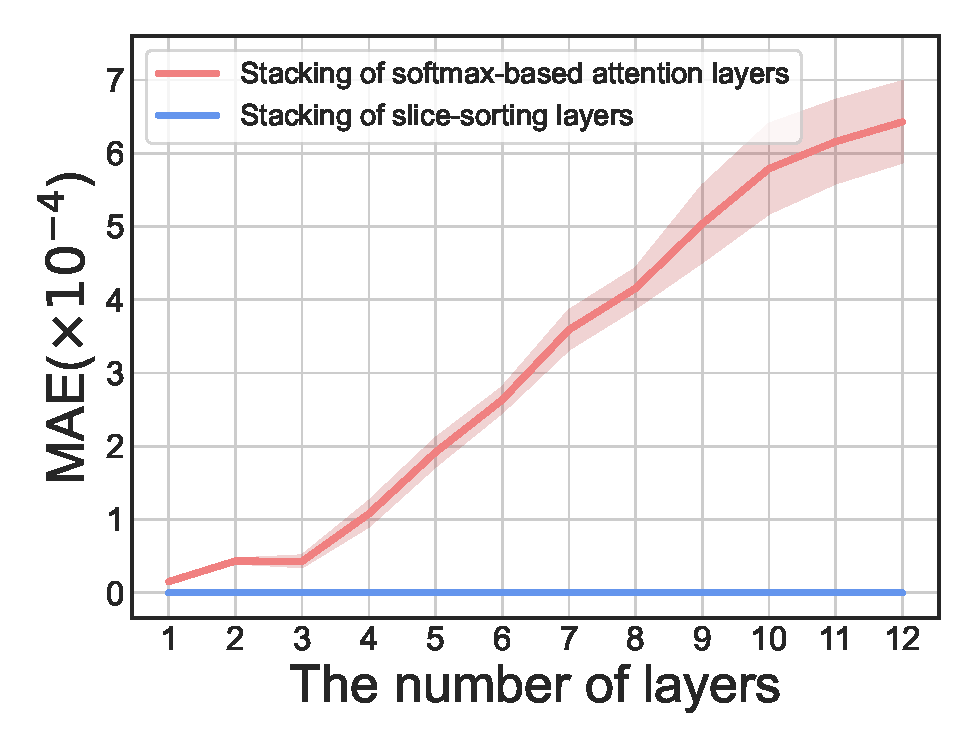
\includegraphics[height=4.3cm]{figures/MAE.pdf}\label{fig:cos}
  }
  \subfigure[Convergence of training process]{
  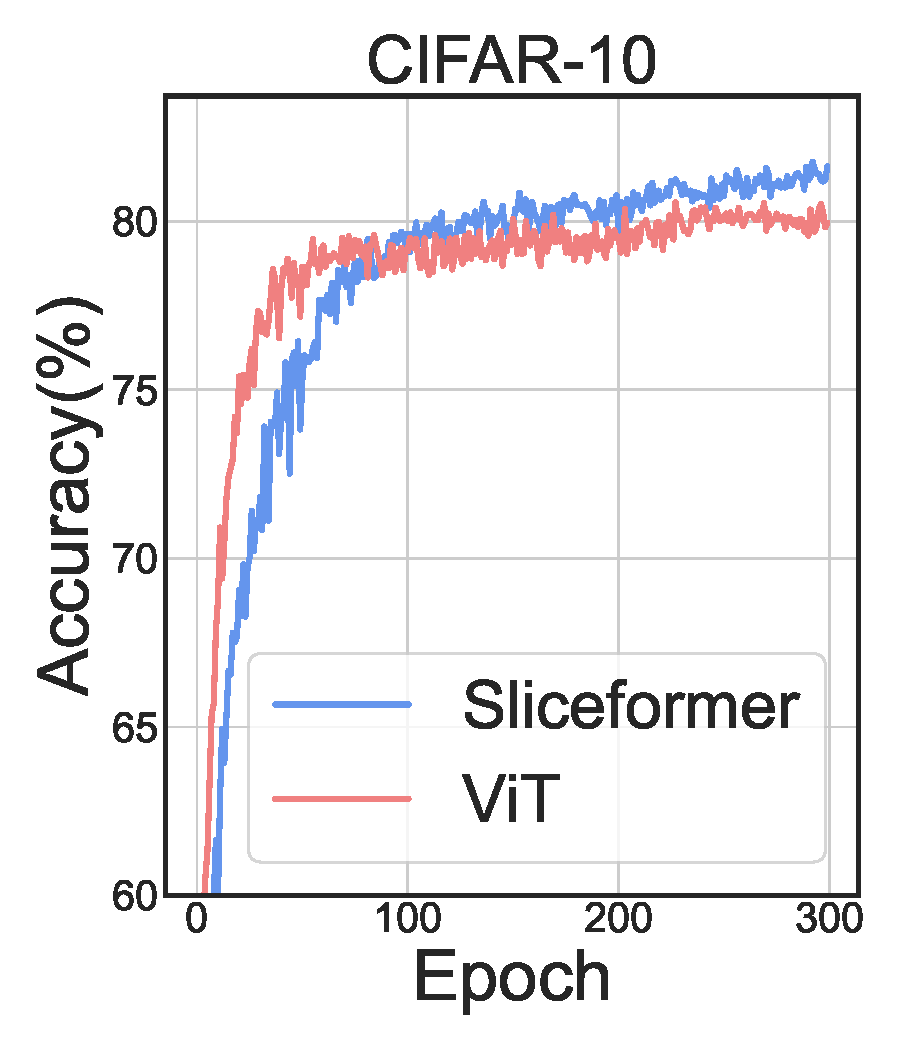
\includegraphics[height=4.5cm]{figures/converge_cifar10.pdf}\label{fig:convergence}
  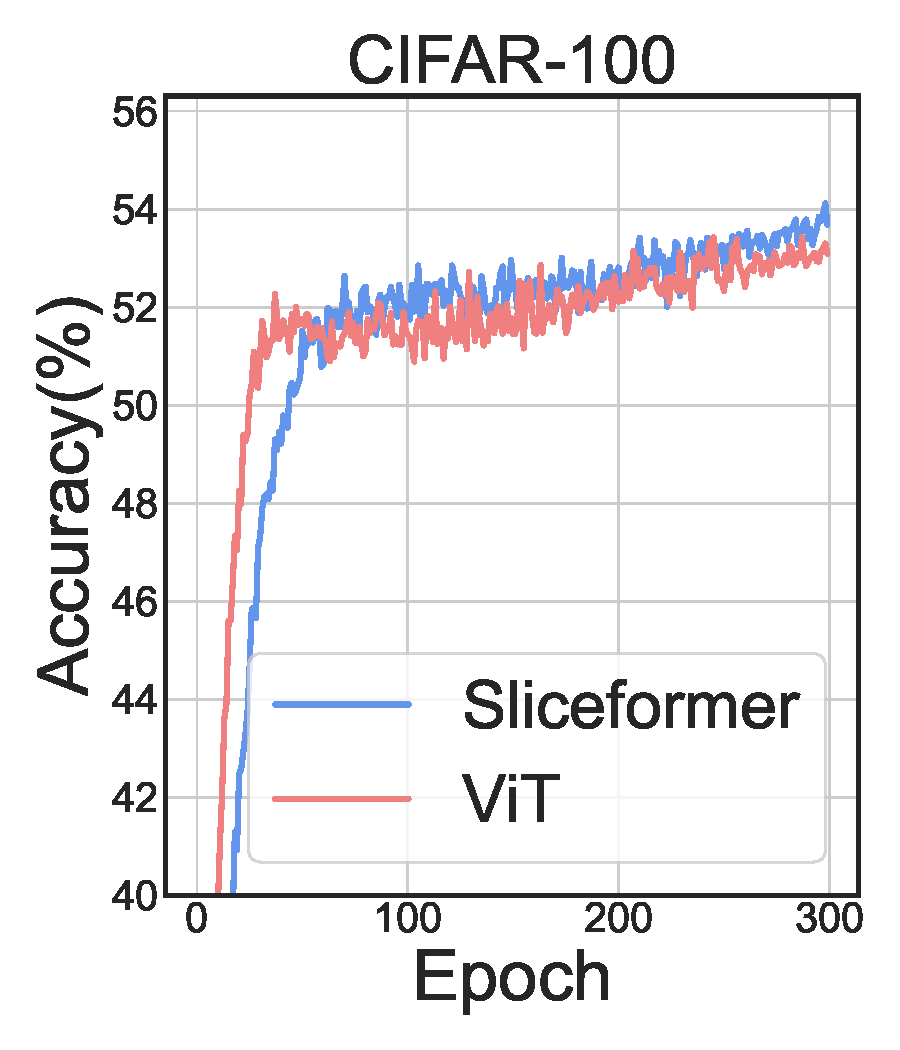
\includegraphics[height=4.5cm]{figures/converge_cifar100.pdf}\label{fig:convergence}
  }
  \caption{
  (a) The impact of the order of pixel sequence on the numerical permutation-invariance of model.
  (b) The comparison for our Sliceformer and ViT on their convergence when training on the CIFAR-10 and CIFAR-100 dataset.
  }
\end{figure}

\textbf{Molecular Analysis.}
Besides achieving a vision Sliceformer, we introduce the slicing-sorting operation to Graphormer~\cite{ying2021transformers} and test its impacts on molecular property prediction. 
In particular, the attention head of Graphormer applies a modified ``query-key-value'' architecture, which is formulated as $\text{Softmax}(\bm{S}+\bm{E}+\frac{1}{\sqrt{D}}\bm{QK}^{\top})\bm{V}$. 
Here $\bm{S}$ and $\bm{E}$ are learnable embedding matrices encoding spatial positions and edge information, respectively. 
% Applying the slicing-sorting operation, we design a simplified attention layer as $\text{Sort}_{\text{col}}(\text{Softmax}(\bm{S}+\bm{E})\bm{V})$, where the query and key matrices are ignored. 
Applying the slicing-sorting operation, we design a simplified attention layer without the query and key matrices and dramatically reduce the trainable parameters by around 30\%.
Replacing the attention layer of Graphormer with this layer leads to a Sliceformer for molecular data.
We apply the PCQM4M-LSC dataset~\cite{hu2021ogb} for training and testing the models. 
The experimental results in Table~\ref{tab:graphormer} show that applying the slicing-sort operation leads to a simplified model with a smaller size, whose performance is comparable to Graphormer.

\section{Conclusion and Future Work}
We have proposed a new data representation model called Sliceformer. 
By replacing the traditional MHA mechanism with a simple slicing-sorting operation, our Sliceformer overcomes the numerical drawbacks of the current Transformers and achieves encouraging performance in various discriminative tasks. 
\textbf{Our work provides a new perspective to the design of the attention layer, i.e., implementing attention maps through simple algorithmic operations has the potential to achieve high model capacity, low computational complexity, and good numerical performance.} 

\textbf{Limitations and Future Work.} 
Currently, the rationality of the proposed model is based on the proposed hypotheses and empirical experiments, and its performance in generative learning tasks is not investigated yet.
Therefore, we would like to find theoretical support for our model and test it in generative learning tasks in the future.
Additionally, beyond the slicing-sorting operation, we plan to develop other better-performing attention layers and apply them to the models for structured data like point clouds and meshes.


\bibliography{refs}
\bibliographystyle{unsrtnat}

\end{document}